\documentclass[titlepage]{article}
\usepackage[utf8]{inputenc}
\usepackage{setspace}
\usepackage[left=1in, right=1in, top=1in, bottom=1in]{geometry}
\usepackage{verbatim}
\usepackage{fancyhdr}
\usepackage{float}
\usepackage{matlab-prettifier}
\usepackage{amssymb}
\usepackage{amsmath}
\usepackage{mathtools}
\usepackage{blindtext}
\usepackage{textcomp}

\usepackage{stackengine}
\stackMath

\usepackage{graphicx}
\graphicspath{ {./figures/} }

\usepackage{xcolor}

\definecolor{codegreen}{rgb}{0,0.6,0}
\definecolor{codegray}{rgb}{0.5,0.5,0.5}
\definecolor{codepurple}{rgb}{0.58,0,0.82}
\definecolor{backcolour}{rgb}{0.95,0.95,0.92}

\lstdefinestyle{mystyle}{
    backgroundcolor=\color{backcolour},   
    commentstyle=\color{codegreen},
    keywordstyle=\color{magenta},
    numberstyle=\tiny\color{codegray},
    stringstyle=\color{codepurple},
    basicstyle=\ttfamily\footnotesize,
    breakatwhitespace=false,         
    breaklines=true,                 
    captionpos=b,                    
    keepspaces=true,                 
    numbers=left,                    
    numbersep=5pt,                  
    showspaces=false,                
    showstringspaces=false,
    showtabs=false,                  
    tabsize=2
}

\lstset{style=mystyle}

\singlespacing
\parindent=0in

\title{ME 577 Final Project}
\author{Charles Goble, Cory Anderson-Wilson, Andy Edgell, \& Eddie Turner}
\date{\today}
\cfoot{Page \thepage}

\begin{document}
\maketitle
\tableofcontents

\newpage
\section{Introduction}
The inverted pendulum on a cart problem is an interesting engineering problem for a multitude of reasons. It serves as the basis for both real and surrogate systems. Companies such as Segway\texttrademark have a self-balancing system marketed as a personal transportation device for urban environments. In this instance, the inverted pendulum on a cart has been actualized into a physical product and sold to the masses. However, the more common realization of the inverted pendulum on a cart problem is a surrogate model for a more complicated dynamical system. NASA has published research showing how the inverted pendulum on a cart problem acts as a rocket in flight and the derived controller can be used to design a control law for a launch vehicle. Finally, the most widely used application of the inverted pendulum on a cart problem is in academia where academics mentor their students in a variety of controls topics using the non-stable but controllable dynamics system to highlight keep concepts in controls engineering.\\

This report follows in the latter example of the utilization for the inverted pendulum on a cart. The inverted pendulum on a cart is the dynamical system for the University of Alabama ME 577: Advanced Linear Control course final project. Contained within this report, the read will find a derivation and linearization of the dynamical system, two controller designs and finally some system response analysis testing the controllers.

\section{Dynamics Derivation}
To start the derivation of the equations of motion, we first need to split the inverted pendulum on a cart into separate components and draw a free body diagram of each.

\begin{figure}[H]
\center
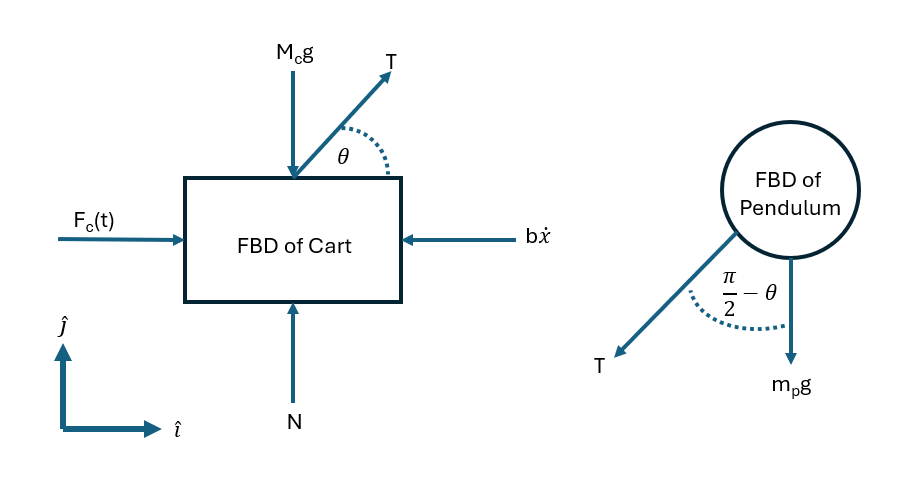
\includegraphics[width=10cm, height=5cm]{free_body_diagram.png}
\caption{Free Body Diagrams of Individual Components}
\end{figure}

As shown in Figure 1, the individual forces action on the cart are the weight, an external control force, a friction damping force, the normal force from the road and a tension force from the rod connecting the pendulum to the cart. The only forces acting on the pendulum are the same rod tension force and the weight of the pendulum. To first step will be to sum all the forces along each coordinate axis for the cart and pendulum.\\

\underline{Cart Forces:}
\begin{equation}
\sum{}{F_{\hat{i}}} = f_{c}\left(t\right) = M_{c}\ddot{x} + b\dot{x} + T\cos{\theta}
\end{equation}
\[ \sum{}{F_{\hat{j}}} = f_{c}\left(t\right) = N - M_{c}g + - T\sin{\theta} = M_{c}\ddot{y}=0 \]

Since the cart is not able to travel in the \(\hat{j}\) direction, the second force summation equation for the cart is mainly shown for completeness. It will be unused in the derivation. If we were interested in quantifying the Normal force acting up on the cart from the road we would use it, however that is not necessary.\\

\underline{Pendulum Forces:}
\[ \sum{}{F_{\hat{i}}} = -T\cos{\theta} = m_{p}a_{p_{x}}\]
\[ \sum{}{F_{\hat{j}}} =  -T\sin{\theta} -m_{p}g = m_{p}a_{p_{y}} \]

In the pendulum equations, a new term has been identified, \(a_{p}\) which acts in both the \(\hat{i}\) and the \(\hat{j}\) directions. This is the acceleration of the pendulum and becomes a force when multiplied by the mass of the pendulum. To compute the acceleration of the pendulum we will use the following equation:

\[a_p = a_c + a_{p/c}\]

where \(a_p\) is the desired acceleration of the pendulum, \(a_c\) is the acceleration of the cart and \(a_{p/c}\) is the acceleration of the pendulum relative to the cart. Defining the acceleration of the cart is easy, it is simply \(a_c=\ddot{x}\hat{i}\). To determine the relative acceleration, we need to use the transport theorem and place a rotating frame on the pendulum and map the acceleration back to our previously defined inertial frame.

\begin{figure}[H]
\center
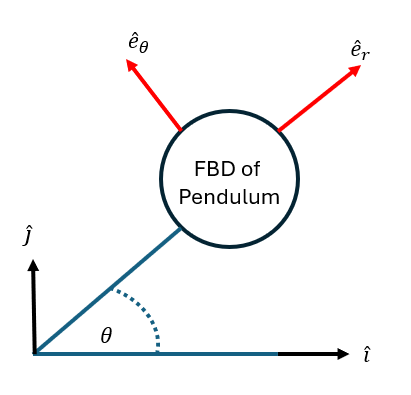
\includegraphics[width=8cm, height=8cm]{rotating_frame.png}
\caption{Pendulum Rotating Coordinate System}
\end{figure}

To compute the desired acceleration, we will use kinematics and start with a position definition for the pendulum in the rotating frame and then take two derivatives using the transport theorem to compute the relative acceleration back to the inertial frame.

\[r = L\hat{e_{r}}\]
\[\dot{r}^{n} = \dot{r}^{b} + \omega_{p/c} \times r = L\dot{\theta}\hat{e_{\theta}}\]
\[\ddot{r}^{n} = \ddot{r}^{b} + \omega_{p/c} \times \dot{r} = L\ddot{\theta}\hat{e_{\theta}} - L\dot{\theta}^{2}\hat{e_{r}}\]

We now have the relative acceleration of the pendulum to the cart in the pendulum's rotating frame. It is a simple transformation to go from the rotating polar coordinate system to the inertial cartesian coordinate system.
\[\hat{e_{r}} = \cos{\theta} \hat{i} + \sin{\theta} \hat{j}\]
\[\hat{e_{\theta}} = -\sin{\theta} \hat{i} + \cos{\theta} \hat{j}\]

Bringing all this together yields the following equation for the acceleration of the pendulum

\begin{equation}
a_p = \left[\ddot{x} -L\ddot{\theta}\sin{\theta} - L\dot{\theta}^{2}\right]\hat{i} + \left[L\ddot{\theta} - L\dot{\theta}\sin{\theta}\right]\hat{j}
\end{equation}

Equation two will now be inserted into the previously defined equations for the pendulum.

\begin{equation}
\sum{}{F_{\hat{i}}} = -T\cos{\theta} = m_{p}\ddot{x} - m_{p}L\ddot{\theta}\sin{\theta} - m_{p}L\dot{\theta}^{2}\cos{\theta}
\end{equation}

\begin{equation}
\sum{}{F_{\hat{j}}} = -T\sin{\theta} - m_{p}g = m_{p}L\ddot{\theta}\cos{\theta} - m_{p}L\dot{\theta}^{2}\sin{\theta}
\end{equation}

As you can see, equations one, three and four all have a variable T representing the tension force between the connecting rod for the cart and pendulum. We need to remove this variable from the equations. To do this, we will first multiple equation (3) by \(\sin{\theta}\) and equation (4) by \(\cos{\theta}\) and then subtract the two equations.

\[-T\cos{\theta}\sin{\theta} = m_{p}\ddot{x}\sin{\theta} - m_{p}L\ddot{\theta}\sin{\theta}^2 - m_{p}L\dot{\theta}^{2}\cos{\theta}\sin{\theta}\]
\[-T\sin{\theta}\cos{\theta} - m_{p}g\cos{\theta} = m_{p}L\ddot{\theta}\cos{\theta}^2 - m_{p}L\dot{\theta}^{2}\cos{\theta}\sin{\theta}\]

\begin{equation}
m_{p}g\cos{\theta} = m_{p}\ddot{x}\sin{\theta} - m_{p}L\ddot{\theta}
\end{equation}

To remove the tension force from equation (1), we will use the tension force found in equation three and substitute it into equation one.

\begin{equation}
T\cos{\theta} = M_{p}L\ddot{\theta}\sin{\theta} + m_{p}L\dot{\theta}^{2}\cos{\theta} - m_{p}\ddot{x}
\end{equation}

Substituting (6) into (1):
\[ f_{c}\left(t\right) = M_{c}\ddot{x} + b\dot{x} +  m_{p}L\ddot{\theta}\sin{\theta} + m_{p}L\dot{\theta}^{2}\cos{\theta} - m_{p}\ddot{x}\]

\begin{equation}
f_{c}\left(t\right) = \left[m_{p} + M_{c}\right]\ddot{x} + b\dot{x} -  m_{p}L\ddot{\theta}\sin{\theta} - m_{p}L\dot{\theta}^{2}\cos{\theta}
\end{equation}

Equations (5) and (7) are the governing non-linear equations of motion in differential form.

\subsection{Linearization}

To start the linearization process, we want to pick one of the two equilibrium conditions for this system. The equilibrium condition of interest, and the unstable but controllable condition, is when the pendulum is vertical at an angle of \(\theta = \pi / 2\).

We are going to now investigate what happens when a small perturbation happens around the equilibrium point.

\[\theta = \frac{\pi}{2} + \Delta\theta\]
\[\cos{\theta} = \cos{\left(\frac{\pi}{2} + \Delta\theta\right)} \approx \Delta\theta\]
\[\sin{\theta} = \sin{\left(\frac{\pi}{2} + \Delta\theta\right)} \approx 1\]

We choose to neglect any squared angle rate term because it will be sufficiently small and always close to zero.

\[\dot{\theta}^{2} \approx 0\]

Implementing these linearization techniques into equation (5) leads to the following set of coupled linear differential equations.

\[m_{p}g\theta = m_{p}\ddot{x} - m_{p}\ddot{\theta}\]
\begin{equation}
\ddot{\theta} = \frac{g}{L}\theta - \frac{1}{L}\ddot{x}
\end{equation}

Similarly, the same linearization process is done on equation (7).

\[\left[m_{p} + M_{c}\right] \ddot{x} = f_{c}\left(t\right) + m_{p}L\ddot{\theta} + b\dot{x}\]

\begin{equation}
\ddot{x} = \frac{b}{2m_{p} + M_{c}}\dot{x} + \frac{m_{p}g}{2m_{p} + M_{c}}\theta + frac{1}{2m_{p} + M_{c}}f_{c}\left(t\right)
\end{equation}

Equation (9) represents the decoupled linear acceleration of the system. However, equation (8) which is the angular acceleration is still a function of the linear acceleration.
The desire is to express the accelerations only in terms of the state variables. Thus, we need to substitute equation (9) into equation (8) to remove the \(\ddot{x}\) term.

\begin{equation}
\ddot{\theta} = -\frac{b}{L\left(2m_{p} + M_{c}\right)}\dot{x} + \left[\frac{g}{L} - \frac{m_{p}g}{2m_{p} + M_{c}}\right]\theta - \frac{1}{L\left(2m_{p} + M_{c}\right)}f_{c}\left(t\right)
\end{equation}

We now have two equations (9) and (10) that represent the linearize decoupled dynamics of the system that are only a function of the state variables and the input control force.

\subsection{State Space Respresentation}

Using the equations developed up to this point, it is rather trivial to put the dynamical system into state space representation form.
Equation (11) and (12) show the state space representation as functions of time.

\begin{equation}
\begin{bmatrix}
\dot{x}\\
\ddot{x}\\
\dot{\theta}\\
\ddot{\theta}\\
\end{bmatrix} =
\begin{bmatrix}
0 & 1  & 0 & 0\\
0 & \frac{b}{2m_{p} + M_{c}}  & \frac{m_{p}g}{2m_{p} + M_{c}} & 0\\
0 & 0  & 0 & 1\\
0 & -\frac{b}{L\left(2m_{p} + M_{c}\right)}  & \frac{g}{L} - \frac{m_{p}g}{L\left(2m_{p} + M_{c}\right)} & 0\\
\end{bmatrix}
\begin{bmatrix}
x\\
\dot{x}\\
\theta\\
\dot{\theta}\\
\end{bmatrix}+ \begin{bmatrix}
0\\
\frac{1}{2m_{p} + M_{c}}\\
0\\
-\frac{1}{L\left(2m_{p} + M_{c}\right)}\\
\end{bmatrix} f_{c}\left(t\right)
\end{equation}

\begin{equation}
\vec{y}\left(t\right) = \begin{bmatrix}
1 & 0  & 0 & 0\\
0 & 1  & 0 & 0\\
0 & 0  & 1 & 0\\
0 & 0  & 0 & 1\\
\end{bmatrix} \begin{bmatrix}
x\\
\dot{x}\\
\theta\\
\dot{\theta}\\
\end{bmatrix} + \begin{bmatrix}
0\\
0\\
0\\
0\\
\end{bmatrix} f_{c}\left(t\right)
\end{equation}

Before showing the controller designs, it is meaningful to show the initial system response from equilibrium inital conditions given a small disturbance of a unit step and a unit impulse.

\begin{figure}[H]
\center
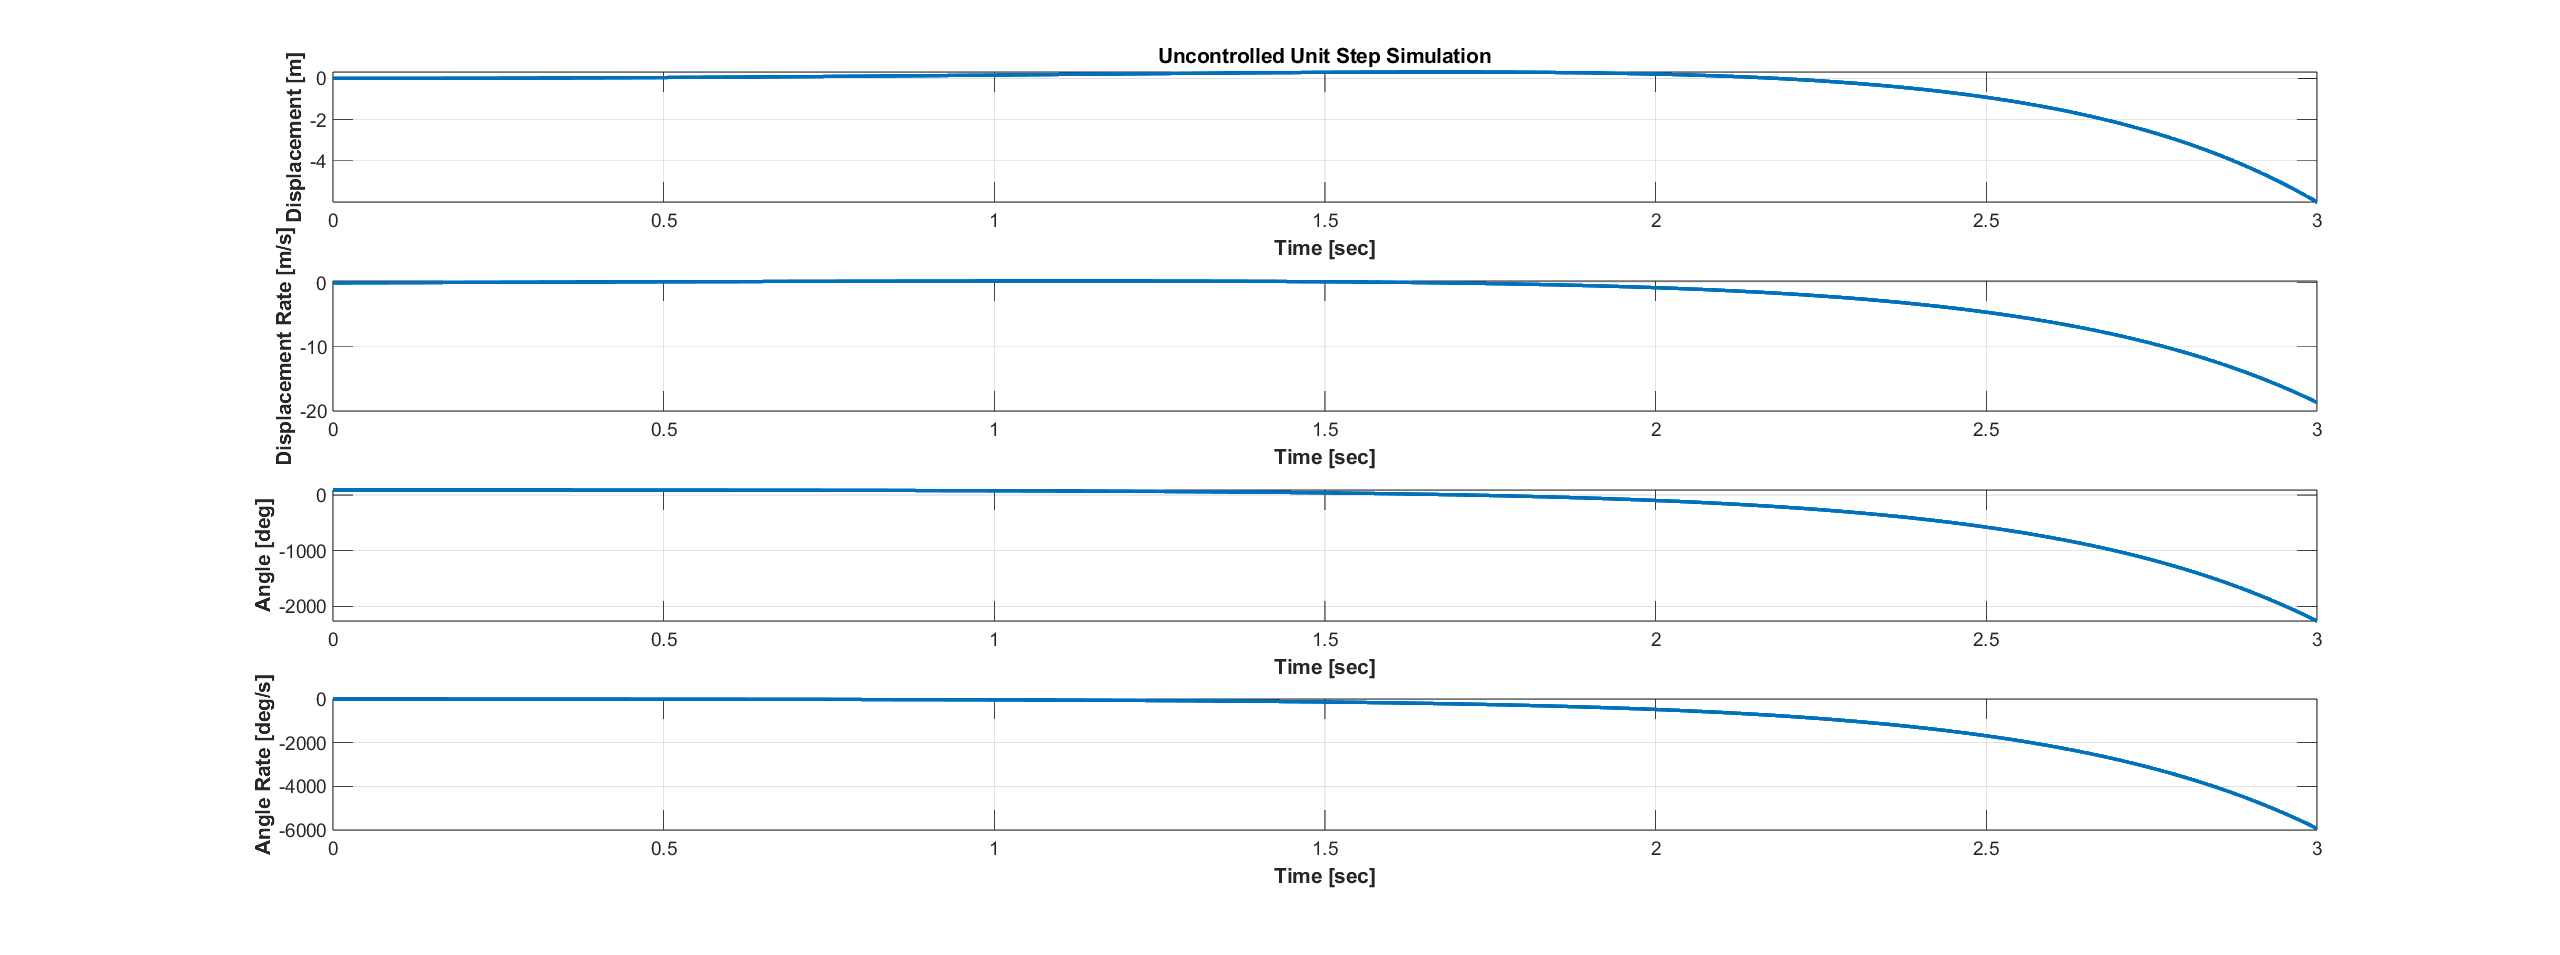
\includegraphics[width=15cm, height=9cm]{uncontrolled_unit_step.png}
\caption{Uncontrolled Inverted Pendulum on Cart Unit Step Simulation}
\end{figure}

\begin{figure}[H]
\center
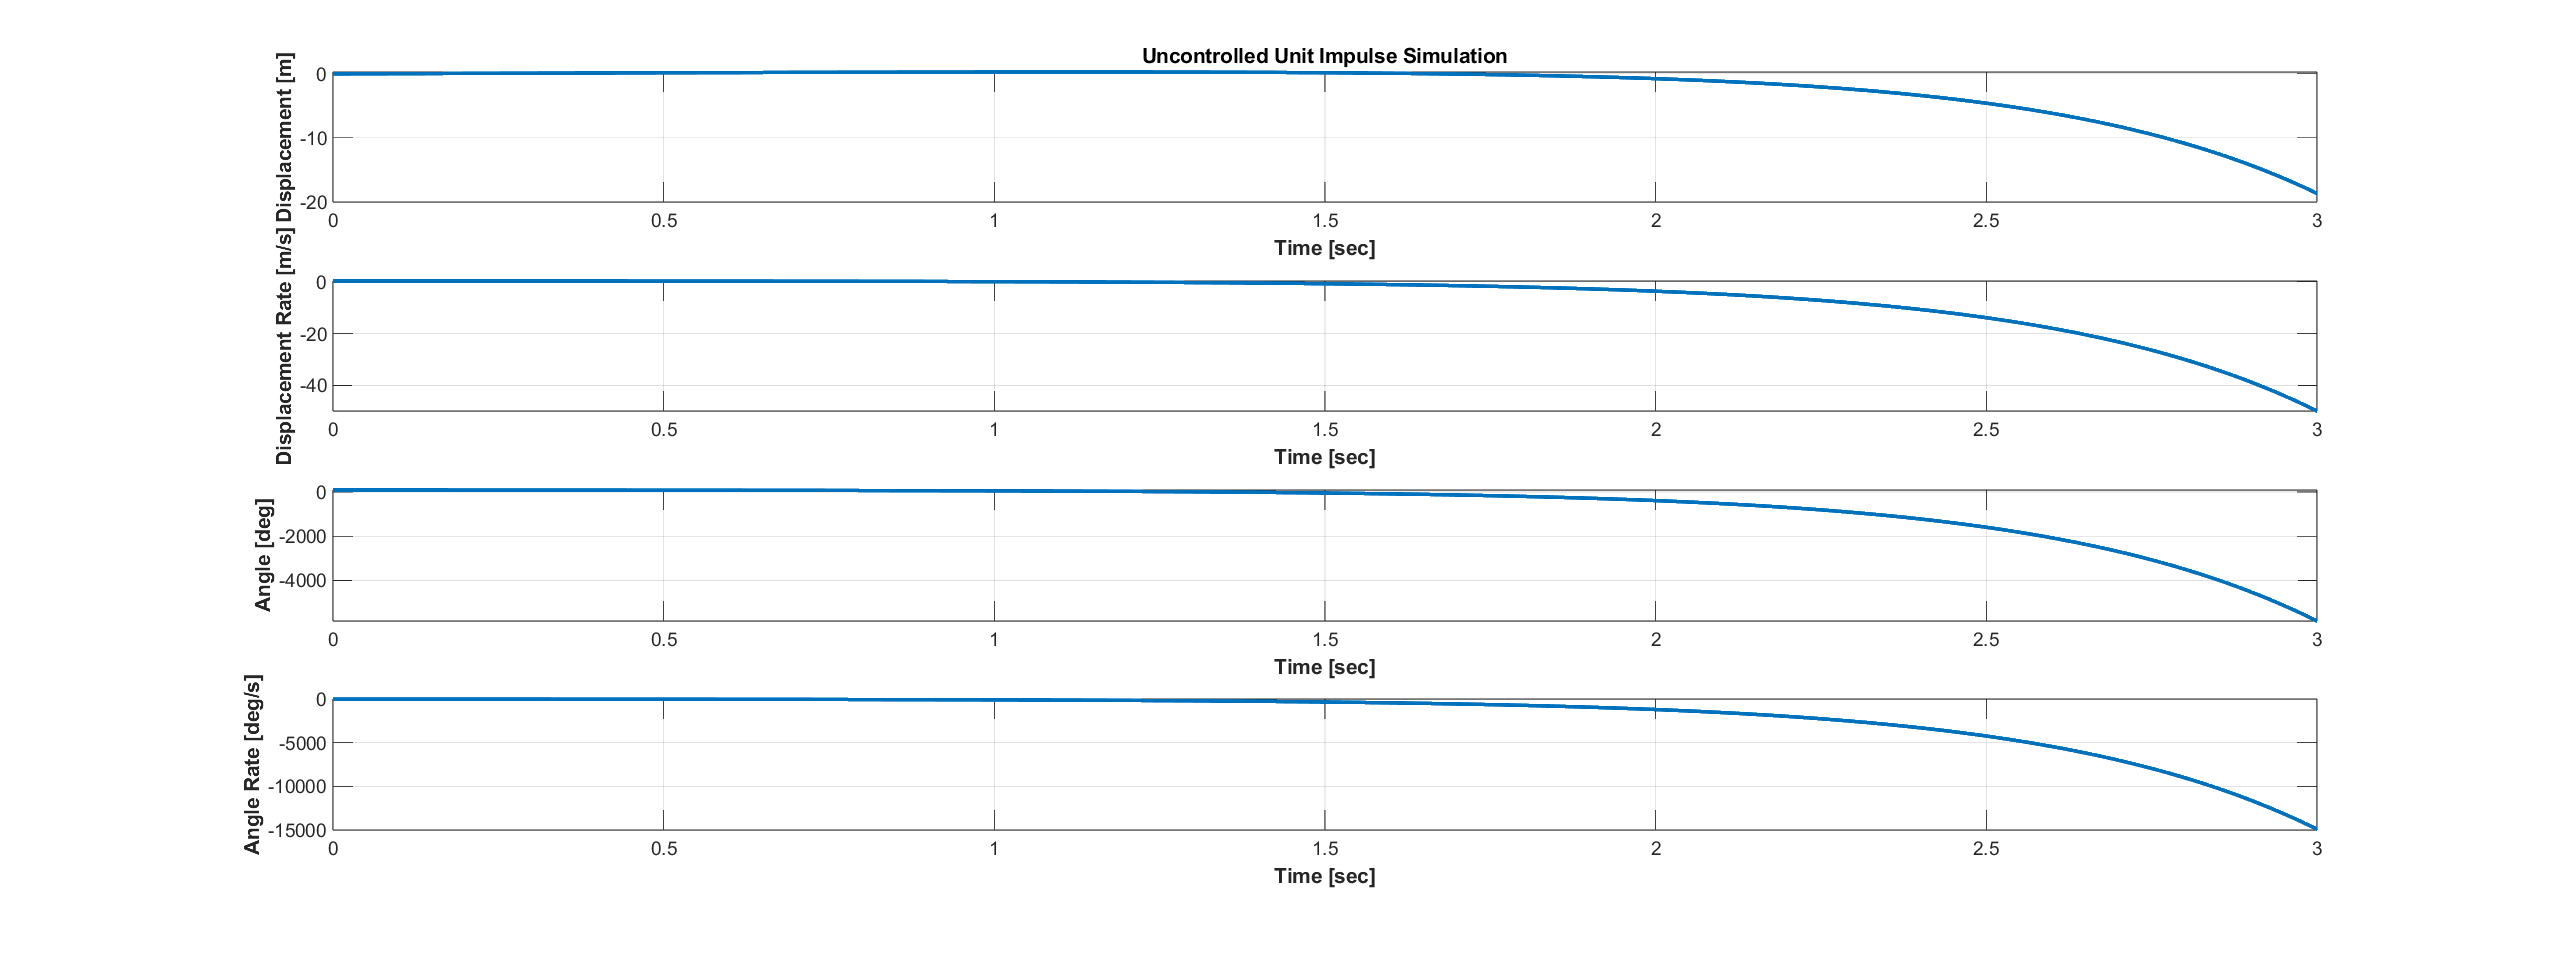
\includegraphics[width=15cm, height=9cm]{uncontrolled_unit_impulse.png}
\caption{Uncontrolled Inverted Pendulum on Cart Unit Impulse Simulation}
\end{figure}

Figures 4 and 5 show that the motion diverges greatly after just a few seconds of simulation due to a unit disturbance. This demonstrates via simulation that the system is not stable and an active controller is necessary to stabilize the system.

\newpage
\section{Close Loop Controller}
	First we want to compute the controllability matrix \textbf{P} and check its rank for control of the system.

	\[\textbf{P} = \begin{bmatrix}
		\textbf{A}^{0}\textbf{B} & \textbf{A}^{1}\textbf{B} & \textbf{A}^{2}\textbf{B} & \cdots & \textbf{A}^{n-1}\textbf{B}\\
	\end{bmatrix}\]

	Controllability is then determined by the rank of \textbf{P}. If the controllability matrix is full rank then the system is controllable, if it is not full rank, then it is not fully controllable.

	For this system, \(n=4\) so the controllability matrix will be of the following format.

	\[\textbf{P} = \begin{bmatrix}
		\textbf{A}^{0}\textbf{B} & \textbf{A}^{1}\textbf{B} & \textbf{A}^{2}\textbf{B}& \textbf{A}^{3}\textbf{B}\\
		\end{bmatrix}\]

	\[\textbf{P} =
	\begin{bmatrix}
		0 & 0.3448 & 0.0297 & -0.3112\\
		0.3448 & 0.0297 & -0.3112 & -0.0539\\
		0 & -0.2653& -0.0229 & -1.6878\\
		-0.2653 & -0.0229 & -1.6878 & -0.1247\\
	\end{bmatrix}\]

	\[rank\left(\textbf{P}\right) = 4\]
	Since \textbf{P} is full rank, the system is controllable.

	Next we want to compute the Observability matrix \textbf{Q} and check its rank for state variables obervation of the system.

	\[\textbf{Q} = \begin{bmatrix}
		\textbf{C}\textbf{A}^{0}\\
		\textbf{C}\textbf{A}^{1}\\
		\textbf{C}\textbf{A}^{2}\\
		\vdots\\
		\textbf{C}\textbf{A}^{n-1}\\
	\end{bmatrix}\]

	Observability is then determined by the rank of \textbf{Q}. If the observability matrix is full rank then the system is fully observable, if it is not full rank, then some of the state variables are not observable.

	For this system, \(n=4\) so the controllability matrix will be of the following format.

	\[\textbf{Q} = \begin{bmatrix}
		\textbf{C}\textbf{A}^{0}\\
		\textbf{C}\textbf{A}^{1}\\
		\textbf{C}\textbf{A}^{2}\\
		\textbf{C}\textbf{A}^{3}\\
		\end{bmatrix}\]

	\[rank\left(\textbf{Q}\right) = 4\]
	Since \textbf{Q} is full rank, the system is fully observable.

	Below is a snippet of the code used to verify these calculations using MATLAB:
	\begin{lstlisting}[style=Matlab-editor]
	%% Stability -> HW 4 type of analysis
	[eigVectors, eigValues] = eig(A);
	linSysPole = pole(linSys);

	%% Controlability -> HW 5 type of analysis
	P = [B, A*B, A*A*B, A*A*A*B];
	rankOfP = rank(P);

	%% Observability -> HW 5 type of analysis
	Q = [C; C*A; C*A*A; C*A*A*A];
	rankOfQ = rank(Q);
	\end{lstlisting}

\subsection{Pole Placement Method}
	To design a controller using the pole placement method we are going to start with the state equations for an open-loop system:
	\[s\vec{X}\left(x\right) = \textbf{A}\vec{X}\left(s\right) + \textbf{B}\vec{U}\left(s\right)\]

	We use the closed-loop definition:
	\[\vec{U}\left(s\right) = \vec{R}\left(s\right) - \textbf{K}\vec{X}\left(s\right)\]

	Substitute the close-loop definition into the open-loop system:
	\[s\vec{X}\left(x\right) = \textbf{A}\vec{X}\left(s\right) + \textbf{B}\vec{U}\left(s\right)\]
	\[s\vec{X}\left(x\right) = \textbf{A}\vec{X}\left(s\right) + \textbf{B}\left[\vec{R}\left(s\right) - \textbf{K}\vec{X}\left(s\right)\right]\]
	\[s\vec{X}\left(x\right) = \left[\textbf{A} - \textbf{B}\textbf{K}\right]\vec{X}\left(s\right) + \textbf{B}\vec{R}\left(s\right)\]

	\textbf{TODO:} Discuss how the closed loop eigen values are calculated.

	Define the characteristic equation to compute \textbf{K}.
	\[\left| s\textbf{I} - \left(\textbf{A} - \textbf{B}\textbf{K}\right)\right| = s^{n} + \left(k_{n}+a_{n-1}\right)s^{n-1}+ \cdots +\left(k_{2}+a_{1}\right)s+\left(k_{1}+a_{0}\right)\]
	For our system:
	\[\left| s\textbf{I} - \left(\textbf{A} - \textbf{B}\textbf{K}\right)\right| = s^{4}+ \left(k_{4}+a_{3}\right)s^{3} + \left(k_{3}+a_{2}\right)s^{2}+ \left(k_{2}+a_{1}\right)s+\left(k_{1}+a_{0}\right)\]
	where
	\[\alpha\left(s\right) = s^{n} + \alpha_{n-1}s^{n-1}+ \cdots +\alpha_{1}s+\alpha_{0}\]
	\[k_{n} = \alpha_{n-1} - a_{n-1}\]
	\[\alpha\left(s\right) = s^{4} + \alpha_{3}s^{3}+ \alpha_{2}s^{2} + \alpha_{1}s +\alpha_{0} = \left(s+\lambda_{1}\right)\left(s+\lambda_{2}\right)\left(s+\lambda_{3}\right)\left(s+\lambda_{4}\right)\]
	\[s^{4} + \alpha_{3}s^{3} + \alpha_{2}s^{2} + \alpha_{1}s +\alpha_{0} =\left(s^3+12s^2+47s+60\right)\]

	\[\textbf{K} = \begin{bmatrix}
		k_1\\
		k_2\\
		k_3\\
		k_3\\
	\end{bmatrix} = \begin{bmatrix}
		1\\
		2\\
		3\\
		4\\
	\end{bmatrix}\]

	Below is a snippet of the code used to compute the \textbf{K} gain matrix using MATLAB:
	\begin{lstlisting}[style=Matlab-editor]
		%% Pole Placement
		zeta = (-1*log(desPO./100))/(sqrt((pi.^2) + (desPO./100)));
		wn = (-1*log(inputPercent./100))./(tSettle.*zeta);
		eqn = [1, 2.1, 3.4, 2.7.*wn, wn.^2];
		p = roots(eqn);
		stableP = p(real(p) == min(real(p)));
		p = [stableP(1); stableP(2);...
		        floor(poleScalarOne*min(real(stableP)));...
		        floor(poleScalarTwo*min(real(stableP)))];

		[K, prec] = place(A, B, p);
		closeLoopA = A - (B*K);
		closeLoopSysPolePlace = ss(closeLoopA, B, C, D);
	\end{lstlisting}

\subsubsection{Unit Step Response}
\begin{figure}[H]
\center
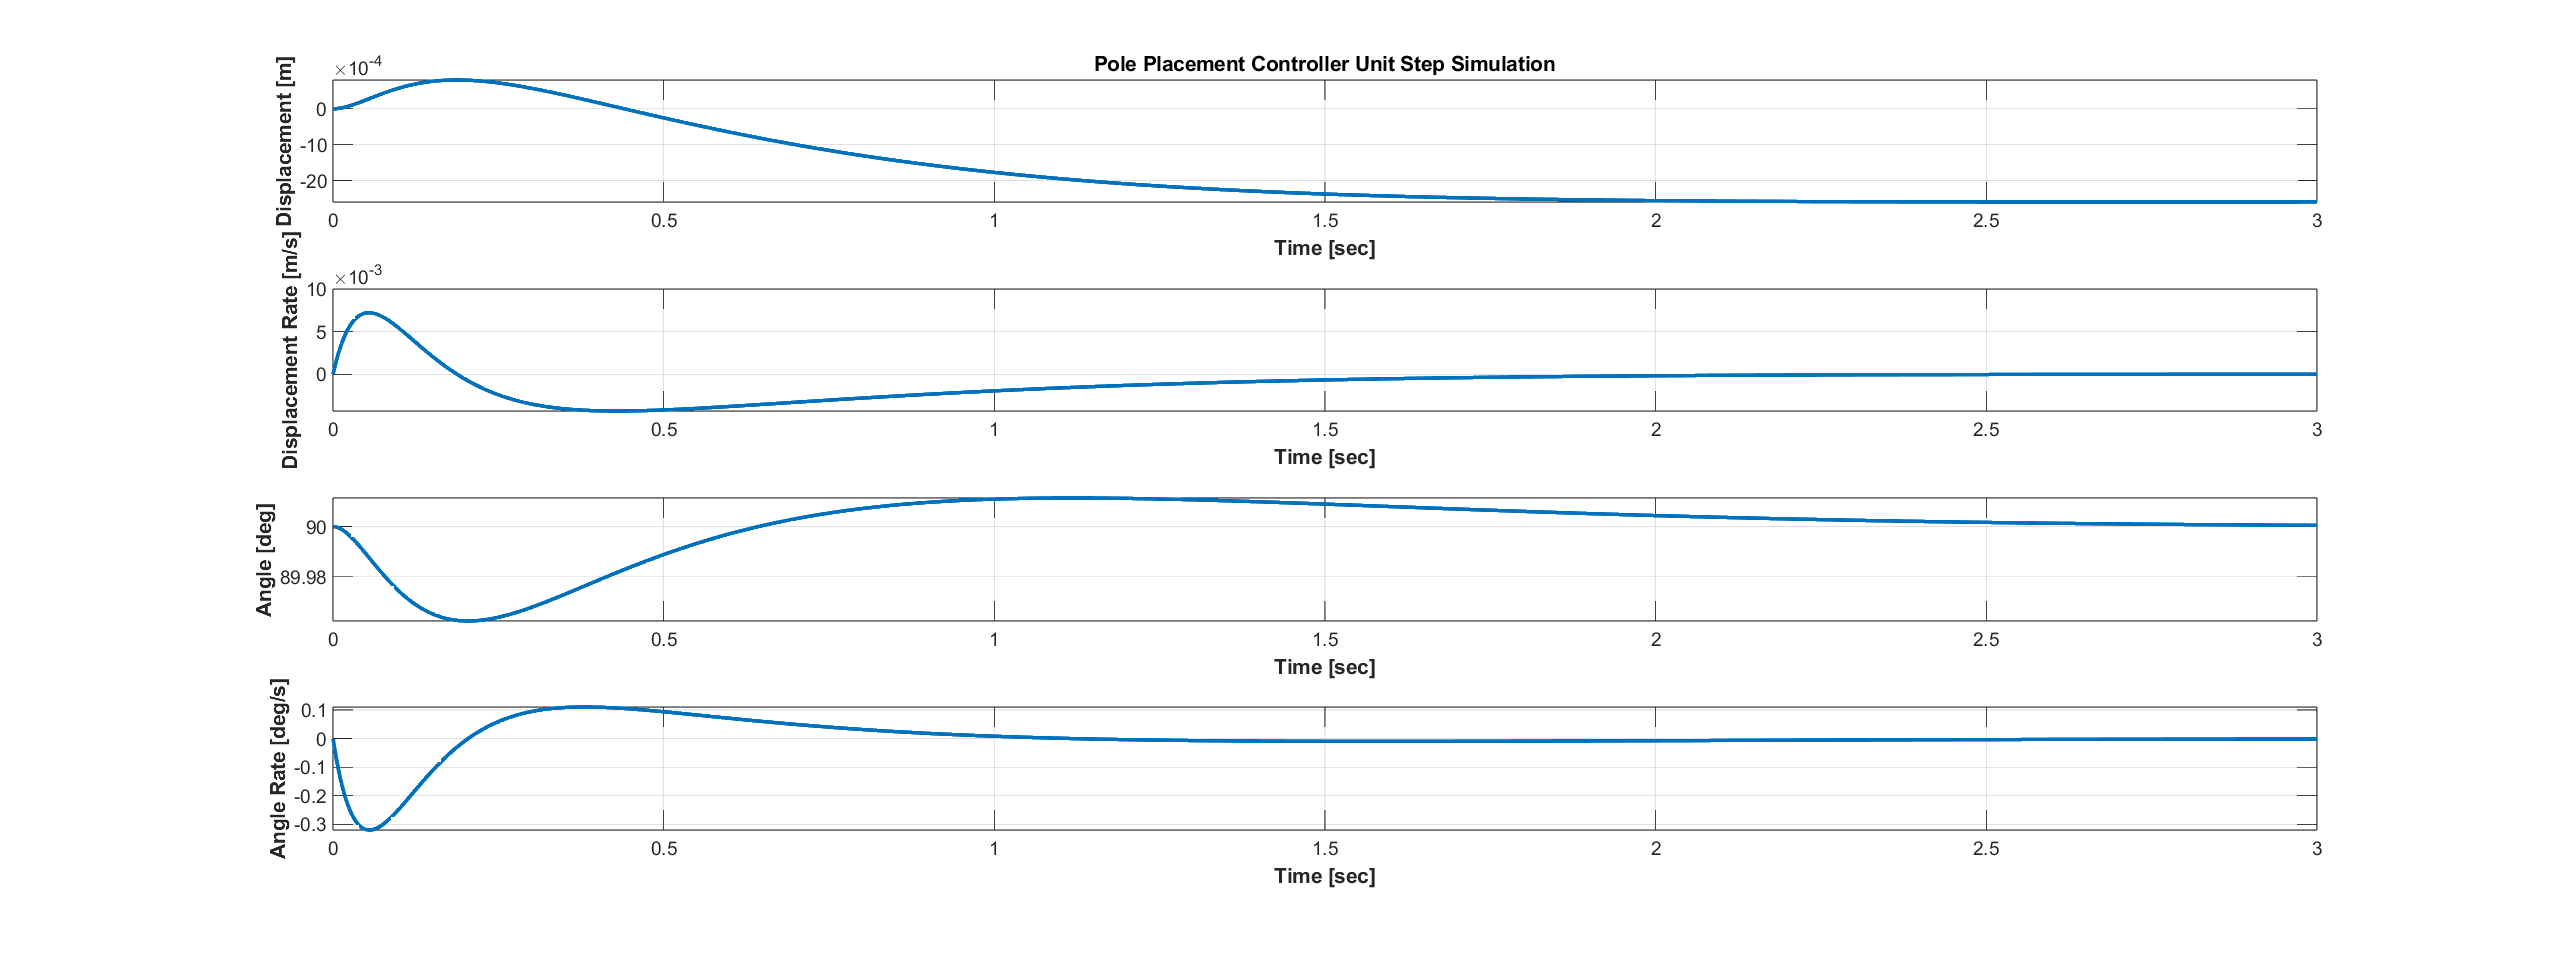
\includegraphics[width=15cm, height=9cm]{pole_placement_unit_step.png}
\caption{Pole Placement Controller Unit Step Disturbance}
\end{figure}

\subsubsection{Unit Impulse Response}
\begin{figure}[H]
\center
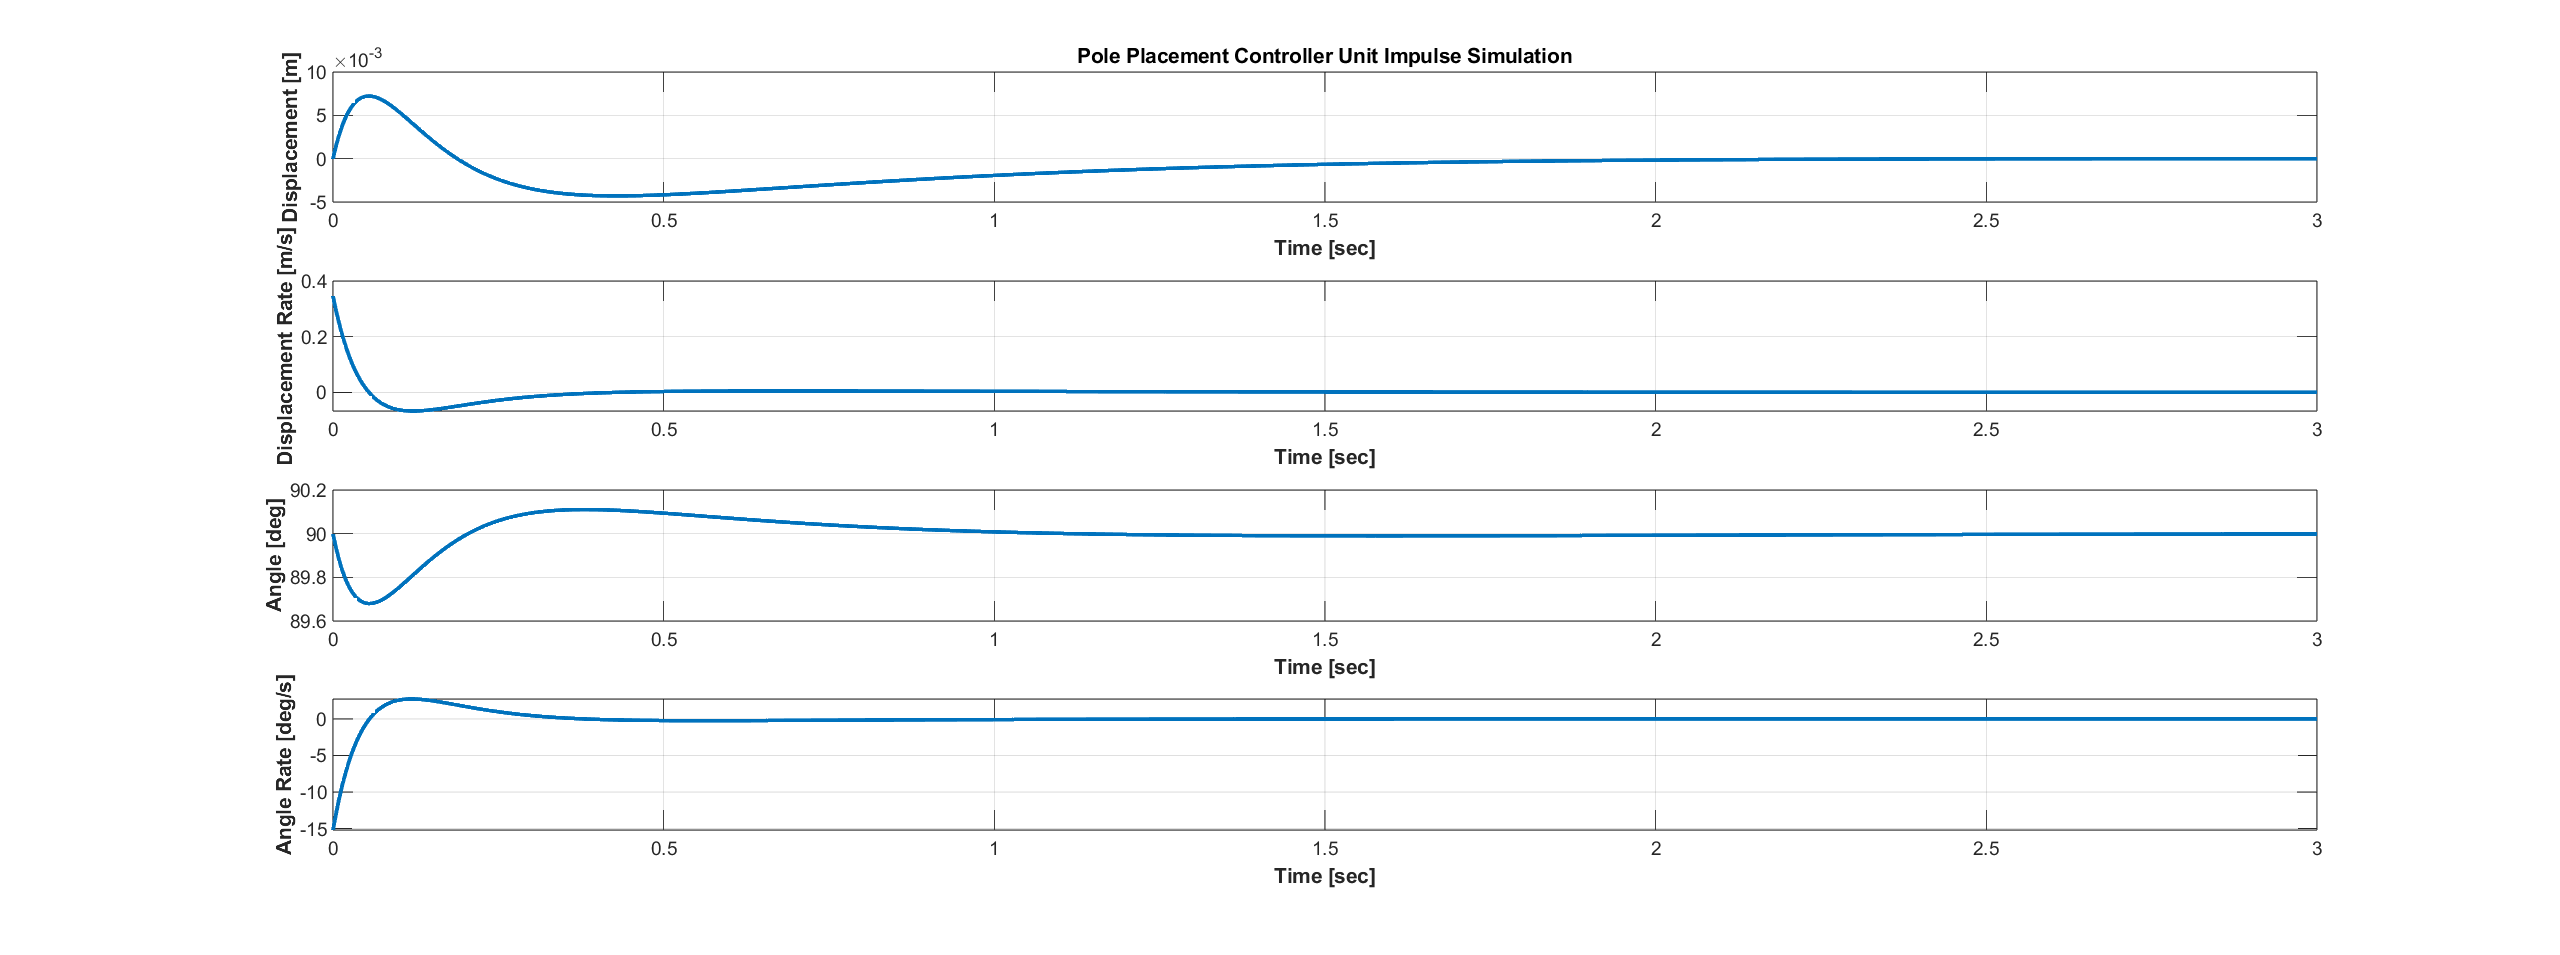
\includegraphics[width=15cm, height=9cm]{pole_placement_unit_impulse.png}
\caption{Pole Placement Controller Unit Impulse Disturbance}
\end{figure}

\subsubsection{Integral Error Controller}
\begin{figure}[H]
\center
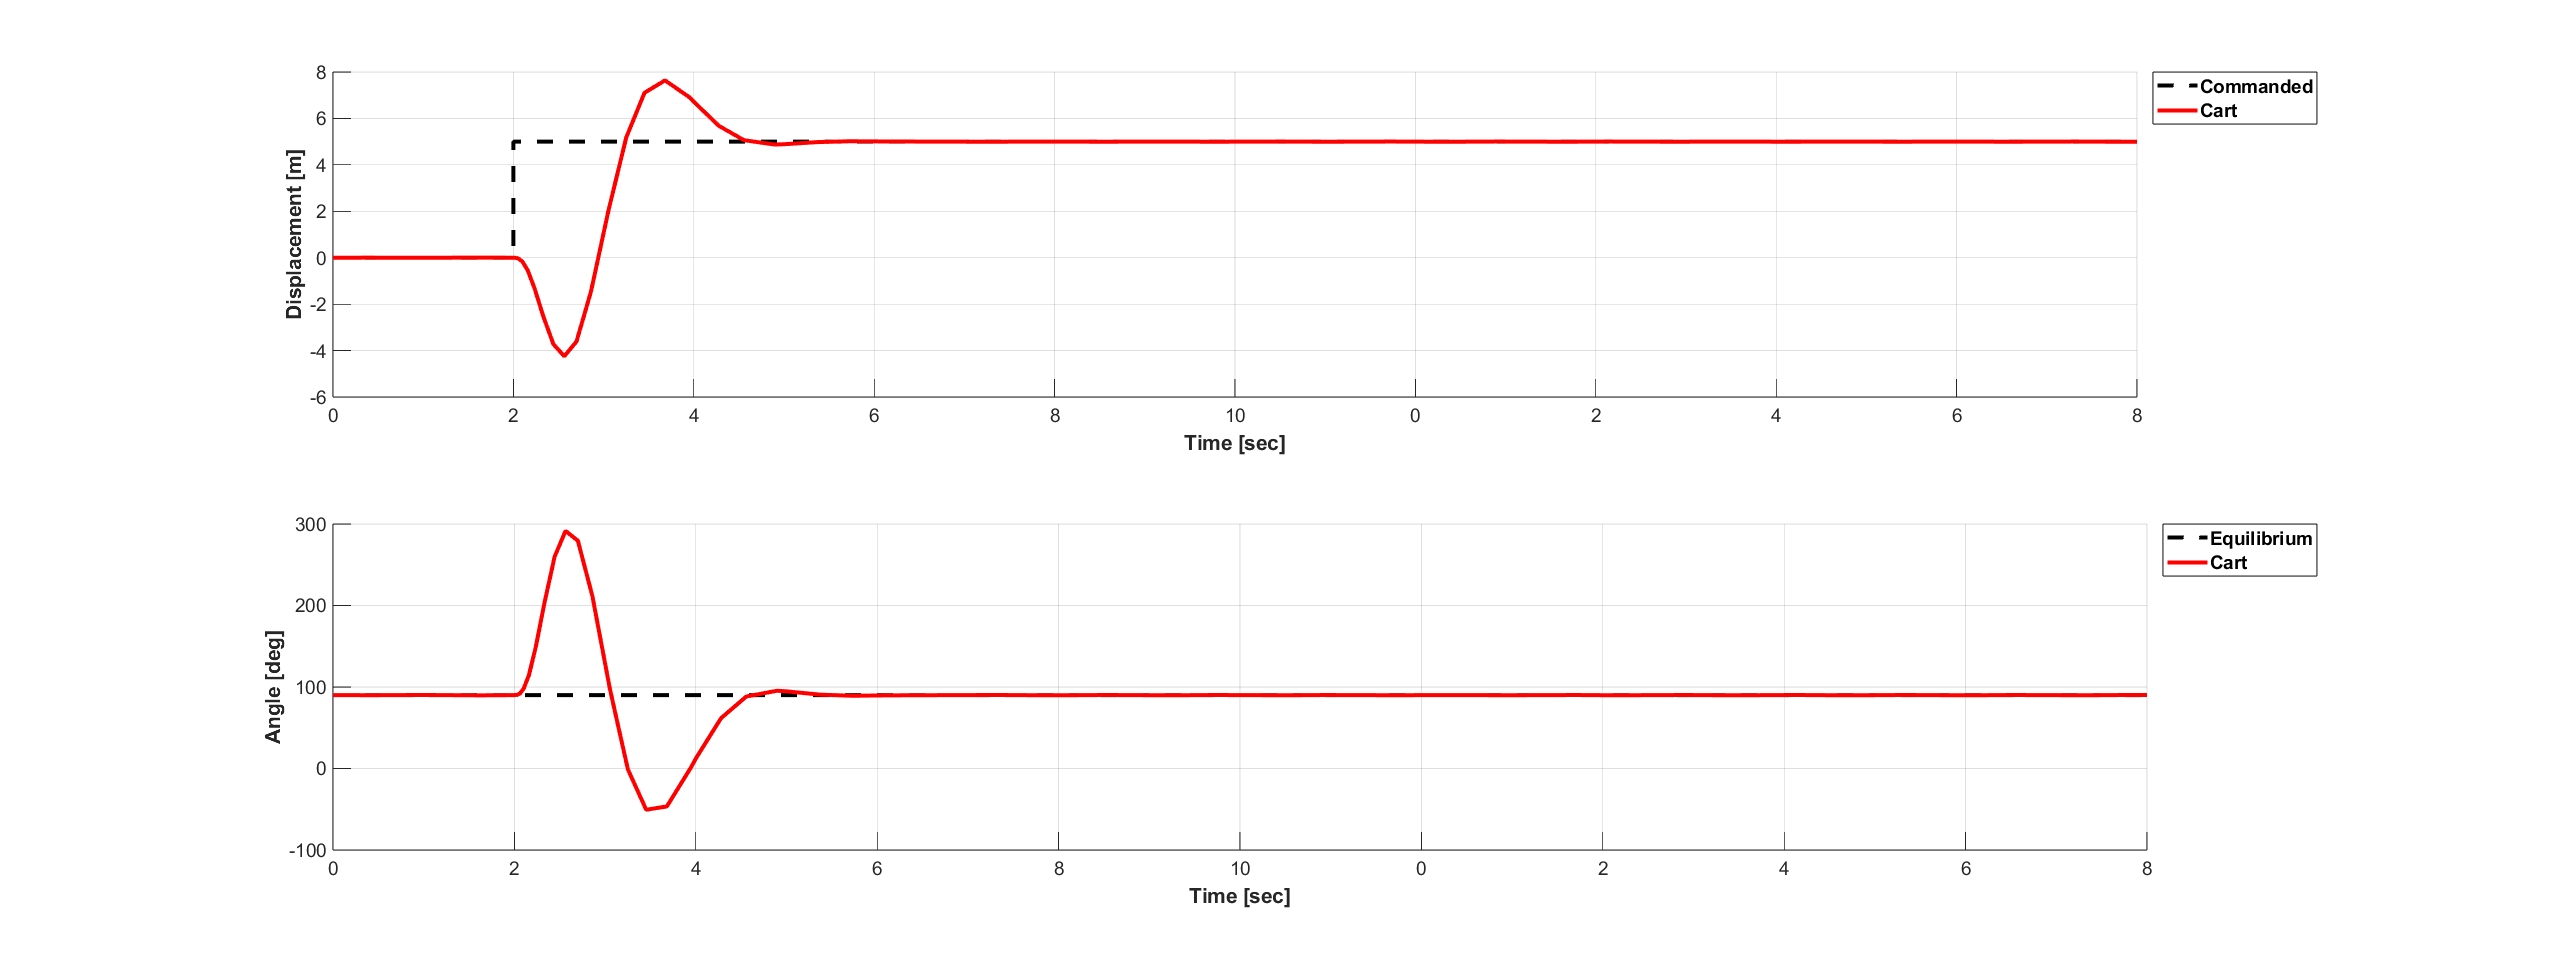
\includegraphics[width=15cm, height=9cm]{pole_placement_integral_error.png}
\caption{Pole Placement Controller Integral Error Control}
\end{figure}

\subsection{LQR}
\subsubsection{Unit Step Response}
\subsubsection{Unit Impulse Response}

\newpage
\section{Response Analysis}

\subsection{Low Frequency Sinusoid Response}

\subsection{High Frequency Sinusoid Response}

\newpage
\section{Conclusion}

\newpage
\section{Appendix A: Source Code}
% Cut and past matlab code here when its all done.
\begin{lstlisting}[style=Matlab-editor]
close all; clear; clc;
%{
ME 577: Advanced Linear Controls
Spring 2025
Final Project
%}

%% Start of Code ...

\end{lstlisting}

\newpage
\section{Appendix B: Simulink}

\newpage
\section{Appendix C: Full Dynamics Derivation}

\end{document}
